\section{Inverse depth and estimation of scatter}
\label{section:dcmSection}
We elaborate on the problem estimating the covariance matrix $\Sigma$ and its eigenvectors and eigenvalues using signed peripherality functions in this section. In addition to conditions (P) and (A1), we assume the following conditions on these functions in this section:

\vspace{1em}
\noindent\textbf{(B1)} The following holds:
$$
P(\bfx; \BF) \leq P(\bfmu_F + t(\bfx - \bfmu_F), \BF),
$$
%
for any $\bfx \in \BR^p$ and $t \in (0,1)$.

\noindent\textbf{(B2)} There exists a positive constant $M(P,\BF) $ such that $P(\bfx; \BF) \rightarrow M(P,\BF)$ as $\|\bfx\| \rightarrow \infty $.
\vspace{1em}

Condition (A2) in Section~\ref{section:LocSection} is now replaced by the stronger condition (B2). Note that all the current conditions are essentially the opposite of those imposed on a traditional depth function \citep{zuo00}. Given a depth function, the peripherality functions in this section can be defined as a bounded monotonically decreasing function of it. Consequently, we use the term {\it inverse depth function} in place of peripherality functions in this section, denoting them by $D^-(\bfx,\BF)$, or equivalently $D^-_\bfX(\bfx)$.

Given an inverse depth function $D^-_{\bfX}(\bfx)$ we transform the original random variable as: $\tilde \bfX = D^-_\bfX(\bfx) \bfS(\bfx - \bfmu)$. We attempt to use these vector as the proxy of original data for improved estimation of the components of the population covariance matrix $\Sigma$ in this section. To this end, in Section~\ref{subsec:dcm} we give some results characterizing the population covariance matrix of these vectors, i.e. $\BV \tilde \bfX$, and its affine equivariant counterpart.

%Data depth is as much a property of a vector-valued random variable $\bfX \in \mathbb{R}^p$ as it is of the underlying distribution $F$, so for ease of notation while working with transformed random variables, from now on we shall be using $D_\bfX(\bfx) = D(\bfx, F)$ to denote the depth of a point $\bfx$. Now, given a depth function $D_{\bfX}(\bfx)$ (equivalently, an htped function $D^-_\bfX(\bfx) = D^-(\bfx, F)$), transform the original random variable as: $\tilde \bfx = \tilde D_\bfX(\bfx) \bfS(\bfx - \bfmu)$, $\bfS(.)$ being the spatial sign functional. The transformed random variable $\tilde \bfX$ can be seen as the multivariate rank corresponding to $\bfX$ (e.g. \cite{serfling2006}). 

%Figure \ref{fig:rankplot} gives an idea of how the multivariate rank vector $\tilde \bfX$ is distributed when $\bfX$ has a bivariate normal distribution. Compared to the spatial sign, which are distributed on the surface of $p$-dimensional unit ball centered at $\bfmu$, these spatial ranks have the same direction as original data and reside \textit{inside} the $p$-dimensional ball around $\bfmu$ that has radius $M_D(F)$ (which, for the case of halfspace depth, equals 0.5).

\subsection{Depth Covariance Matrix}
\label{subsec:dcm}
Consider the spectral decomposition of $\Sigma$: $\Sigma = \Gamma\Lambda\Gamma^T$, $\Gamma$ being orthogonal and $\Lambda$ diagonal with positive diagonal elements $\lambda_1, \ldots, \lambda_p$. Also normalize the original random variable as $\bfZ = \Gamma^T\Lambda^{-1/2} (\bfX - \bfmu)$. In this setup, we can represent the transformed random variable as
%
\begin{eqnarray}
\tilde \bfX &=& D^-_{\bfX} (\bfX) \bfS(\bfx - \bfmu) \notag \\
&=& D^-_{\Gamma\Lambda^{1/2}\bfZ + \bfmu} (\Gamma\Lambda^{1/2} \bfZ + \bfmu). \bfS(\Gamma\Lambda^{1/2} \bfZ) \notag \\
&=& \Gamma D^-_{\bfZ}(\bfZ) \bfS(\Lambda^{1/2}\bfZ) \notag \\
&=& \Gamma \Lambda^{1/2} D^-_{\bfZ}(\bfZ) \bfS(\bfZ) \frac{\| \bfZ \|}{\|\Lambda^{1/2} \bfZ \|}.
\label{equation:rankdecomp}
\end{eqnarray}
%
%Because of affine (thus rotational) invariance of a depth function, the depth (htped) value at $\bfz$ does not depend on the direction of $\bfz$, i.e. $D^-_{\bfZ}(\bfz)$ and $\bfS(\bfz)$ are independent. Furthermore,
%$$ Cov \left(\bfS (\bfz), \frac{\| \bfz \|}{\|\Lambda^{1/2} \bfz\|} \right) = E \left(\bfS (\bfz). \frac{\| \bfz \|}{\|\Lambda^{1/2} \bfz\|} \right) - E \bfS (\bfz) E \left(\frac{\| \bfz \|}{\|\Lambda^{1/2} \bfz\|} \right) = E \left( \frac{\bfz}{\|\Lambda^{1/2} \bfz\|} \right) = \bf0$$
%both $\bfS (\bfz)$ and $\bfz / \| \Lambda^{1/2}\bfz \|$ are odd functions of $\bfz$, which has a circularly symmetric distribution, hence each of them has expectation $\bf0$. Consequently, we obtain an expression for the covariance matrix of $\tilde \bfX$:

$D^-_\bfZ(\cdot)$ is an even function in its argument because of affine invariance, as is $\| \bfz \| / \|\Lambda^{1/2} \bfz \|$. Since the sign function $\bfS(\cdot)$ is odd in its argument, it follows that $\BE \tilde \bfX = \bf0$. Consequently, we obtain an expression for $\BV \tilde \bfX$, which we call the {\it Depth Covariance Matrix} (DCM):

\begin{Theorem} \label{Theorem:covform}
Let the random variable $\bfX \in \mathbb{R}^p$ follow an elliptical distribution with center $\bfmu$ and covariance matrix $\Sigma = \Gamma\Lambda\Gamma^T$, its spectral decomposition. Then, given a depth function $D_\bfX(.)$ the covariance matrix of the transformed random variable $\tilde\bfX$ is
\begin{equation} \label{equation:covformEq1}
\BV \tilde \bfX) = \Gamma \Lambda_{D} \Gamma^T,\quad\mbox{with}\quad \Lambda_{D} = \mathbb E_\bfZ \left[ (D^-_\bfZ(\bfz))^2 \frac{\Lambda^{1/2} \bfz \bfz^T \Lambda^{1/2}}{\bfz^T \Lambda \bfz} \right],
\end{equation}
where $\bfZ = (Z_1,...,Z_p)^T \sim N({\bf 0}, \bfI_p)$, so that $\Lambda_{D}$ a diagonal matrix with diagonal entries
%
$$
\lambda_{D,i} = \mathbb E_\bfZ \left[ \frac{(D^-_\bfZ(\bfz))^2 \lambda_i z_i^2}{\sum_{j=1}^p \lambda_j z_j^2} \right].
$$
\end{Theorem}

The matrix of eigenvectors $\Gamma$ remains unchanged in the transformation $\bfX \rightarrow \tilde \bfX$. As a result, the multivariate rank vectors can be used for robust principal component analysis, which we are going to discuss shortly. However, as one can see in the above expression, the diagonal entries of $\Lambda_{D}$ do not change if a scale change is done on all entries of $\Lambda$, meaning the $\Lambda_{D}$ matrices corresponding to $\BF$ and $c \BF$ for some $c \neq 0$ will be same. This is the reason the DCM is not equivariant under affine transformations.

We need to follow the general framework of M-estimation with data-dependent weights \citep{HuberBook81} to construct an affine equivariant counterpart of the DCM. Specifically, we implicitly define the Affine-equivariant Depth Covariance Matrix (ADCM) as
%
\begin{equation} \label{eqn:ADCM}
\Sigma_{Dw} = \frac{1}{ \BV \tilde Z_1 } \BE_\bfX \left[ \frac{(D^-_\bfX(\bfx))^2 (\bfx - \bfmu) (\bfx - \bfmu)^T}{(\bfx - \bfmu)^T \Sigma_{Dw}^{-1} (\bfx - \bfmu)} \right].
\end{equation}
%
Its affine equivariance follows from the fact that the weights $(D^-_\bfX (\bfx))^2$ depend only on the standardized quantities $\bfz \sim \cE ({\bf 0}, k \bfI_p, g)$. We solve (\ref{eqn:ADCM}) iteratively by obtaining a sequence of positive definite matrices $\Sigma^{(k)}_{Dw}$ until convergence:
%
$$
\Sigma^{(k+1)}_{Dw} = \frac{1}{\BV \tilde Z_1 } \BE_\bfX \left[ \frac{(D^-_\bfX(\bfx))^2 (\Sigma^{(k)}_{Dw})^{1/2} (\bfx - \bfmu) (\bfx - \bfmu)^T (\Sigma^{(k)}_{Dw})^{1/2}}{(\bfx - \bfmu)^T (\Sigma^{(k)}_{Dw})^{-1} (\bfx - \bfmu)} \right].
$$
%

To ensure existence and uniqueness of this estimator, let us consider the class of scatter estimators $\Sigma_M$ that are obtained as solutions of the following equation:
%
\begin{equation}
E_{\bfZ_M} \left[ u( \| \bfz_M \| )  \frac{\bfz_M \bfz_M^T}{\| \bfz_M \|^2}  - v( \| \bfz_M \| ) I_p \right] = 0
\end{equation}
%
with $\bfz_M = \Sigma_M^{-1/2} (\bfx - \bfmu)$. Under the following assumptions on the scalar valued functions $u$ and $v$, the above equation produces a unique solution \citep{HuberBook81}:
%

\vspace{1em}
\noindent\textbf{(M1)} The function $u(r)/r^2$ is monotone decreasing, and $u(r)>0$ for $r>0$;

\noindent\textbf{(M2)}  The function $v(r)$ is monotone decreasing, and $v(r)>0$ for $r>0$;

\noindent\textbf{(M3)} Both $u(r)$ and $v(r)$ are bounded and continuous;

\noindent\textbf{(M4)} $u(0) / v(0) < p$;

\noindent\textbf{(M5)} For any hyperplane in the sample space $\mathcal X$, (i) $P(H) = E_\bfX 1_{\bfx \in H} < 1 - p v(\infty) / u(\infty)$ and (ii) $P(H) \leq 1/p$.
%

\vspace{1em}
\noindent In our case we take $v(r) = Var(\tilde Z_1)$, i.e. a constant, thus (M2) and (M3) are trivially satisfied. As for $u$, we notice that most well-known depth functions can be expressed as simple functions of the norm of the standardized random variable. For example, $PD_\bfZ (\bfz) = (1 - G(\| \bfz \|); MhD_\bfZ (\bfz) = (1+\| \bfz \|^2)^{-1}; HSD_\bfZ (\bfz) = (1+\| \bfz \|)^{-1}$ etc., so that we can take as $u$ square of the corresponding peripherality functions:
% Var(Z1) breaks into two independent parts: depth and sign. So can check m4 and M5 here itself.
$$
u_{PD} (r) = G^2 (r); \quad u_{MhD}(r)  = \frac{r^4}{(1 + r^2)^2}; \quad u_{HSD}(r)  = \frac{r^2}{(1 + r/G^{-1}(0.75))^2}
$$
%

It is easy to verify that the above choices of $u$ satisfy (M1) and (M3). To check (M4) and (M5), first notice that $\bfZ$ has a spherically symmetric distribution, so that its norm and sign are independent. Since $D_\bfZ(\bfz)$ depends only on $\| \bfz \|$, we have
%
$$
Var (\tilde Z_1) = Var \left( D^-_\bfZ (\bfZ) \frac{Z_1}{ \|\bfZ \|} \right) = Var (D^-_\bfZ (\bfZ)) Var (S_1 (\bfZ)) = \frac{1}{p} Var (D^-_\bfZ (\bfZ))
$$
%
as $Cov(\bfS(\bfZ)) = Cov((S_1(\bfZ), S_2(\bfZ), ..., S_p(\bfZ))^T) = I_p/p$. Now for MhD and HSD $u(\infty)=1, u(0)=0$, so (M4) and (M5) are immediate. To achieve this for PD, we only need to replace $u_{PD}(r)$ with $u_{PD}^*(r) = G^2(r) - 1/4$.

\subsection{Calculating the sample DCM and ADCM}
Let us now consider $n$ iid random draws from our elliptic distribution $F$, say $\bfX_1,...,\bfX_n$. For ease of notation, denote $SS(\bfx; \bfmu) = \bfS(\bfx - \bfmu) \bfS(\bfx - \bfmu)^T$. Then, given the depth function and known location center $\bfmu$, one can show that the vectorized form of $\sqrt n$-times the sample DCM: $\sum_{i=1}^n (D^-_\bfX(\bfx_i))^2SS(\bfx_i; \bfmu) /\sqrt{n}$  has an asymptotic multivariate normal distribution with mean $\sqrt n.vec(E[( (D^-_\bfX (\bfX))^2 SS(\bfx; \bfmu)])$ and a certain covariance matrix by straightforward application of the central limit theorem (CLT). But in practice the population depth function $D_\bfX(\bfx) = D(\bfx, F)$ is estimated by the depth function based on the empirical distribution function, $F_n$. Denote this sample depth by $D^n_\bfX (\bfx) = D(\bfx, F_n)$. Here we make the following assumption regarding how it approximates $D_\bfX(\bfx)$:

\vspace{1em}
\noindent\textbf{(D5)} \textit{Uniform convergence}: $\sup_{\bfx \in \mathbb R^p} | D^n_\bfX (\bfx) - D_\bfX (\bfx) | \rightarrow 0$ as $n \rightarrow \infty $.
\vspace{1em}

The assumption that empirical depths converge uniformly at all points $\bfx$ to their population versions holds under very mild conditions for several well known depth functions: for example projection depth \citep{zuo03} and simplicial depth \citep{Dumbgen92}. One also needs to replace the known location parameter $\bfmu$ by some estimator $\hat\bfmu_n$. Examples of robust estimators of location that are relevant here include the spatial median \citep{haldane48,brown83}, Oja median \citep{oja83}, projection median \citep{zuo03} etc. Now, given $D^n_\bfX(.)$ and $\hat \bfmu_n$, to plug them into the sample DCM and still go through with the CLT we need the following result:

\begin{Lemma} \label{Lemma:lemma1}
Consider a random variable $\bfX \in \mathbb{R}^p$ having a continuous and symmetric distribution with location center $\bfmu$ such that $E\|\bfx - \bfmu \|^{-3/2} < \infty$. Given $n$ random samples from this distribution, suppose $\hat\bfmu_n$ is an estimator of $\bfmu$ so that $\sqrt n (\hat\bfmu_n - \bfmu) = O_P(1) $. Then with the above notations, and given the assumption (D5) we have
%
$$ \sqrt n \left[
\frac{1}{n} \sum_{i=1}^n (D^{-n}_\bfX (\bfx_i))^2 SS(\bfx_i; \hat\bfmu_n) -
\frac{1}{n} \sum_{i=1}^n (D^-_\bfX (\bfx_i))^2 SS(\bfx_i; \bfmu) \right]
\stackrel{P}{\rightarrow} 0 $$
\end{Lemma}

Following this, we are now in a position to state the result for consistency of the sample DCM:

\begin{Theorem} \label{Theorem:rootn}
Consider $n$ iid samples from the distribution in Lemma \ref{Lemma:lemma1}. Then, given a depth function $D_\bfX(.)$ and an estimate of center $\hat\bfmu_n$ so that $\sqrt n(\hat \bfmu_n - \bfmu) = O_P(1)$,
%
$$ \sqrt n \left[ vec\left\{ \frac{1}{n} \sum_{i=1}^n (D^{-n}_\bfX (\bfx_i))^2 SS(\bfx_i; \hat\bfmu_n) \right\} - E \left[ vec\left\{ (D^-_\bfX (\bfx))^2 SS(\bfx; \bfmu) \right\} \right] \right]
\stackrel{D}{\rightarrow}
N_{p^2} ({\bf 0}, V_{D,S}(F)) $$
$$ \text{with } V_{D,S}(F) = Var \left[vec \left\{ (D^-_\bfX (\bfx))^2 SS(\bfx; \bfmu) \right\} \right] $$
\end{Theorem}

\noindent In case $F$ is elliptical, an elaborate form of the covariance matrix $V_{D,S}(F)$ explicitly specifying each of its elements (more directly those of its $\Gamma^T$-rotated version) can be obtained, which is given in Appendix \ref{section:appA}. This form is useful when deriving limiting distributions of eigenvectors and eigenvalues of the sample DCM.

In contrast to the DCM, the issue of estimating $\bfmu$ to plug into the ADCM is easily handled by simultaneously solving for the location and scatter functionals ($\bfmu_{Dw}, \Sigma_{Dw}$):
%
\begin{eqnarray}
E \left[ \frac{\Sigma_{Dw}^{-1/2} (\bfx - \bfmu_{Dw})}{ \| \Sigma_{Dw}^{-1/2}(\bfx - \bfmu_{Dw}) \|} \right] &=& {\bf 0}_p \label{eqn:AffineMedian}\\
E \left[ \frac{(D^-_\bfX(\bfx))^2 \Sigma_{Dw}^{-1/2} (\bfx - \bfmu_{Dw}) (\bfx - \bfmu_{Dw})^T \Sigma_{Dw}^{-1/2}}{(\bfx - \bfmu_{Dw})^T \Sigma_{Dw}^{-1} (\bfx - \bfmu_{Dw})} \right] &=& Var (\tilde Z_1) I_p \label{eqn:AffineCov}
\end{eqnarray}
%
In the framework of (\ref{eqn:ADCM}), for any fixed $\Sigma_M$ there exists a unique and fixed solution of the location problem $E_{\bfZ_M} (w(\| \bfz_M \| \bfz_M) = {\bf 0}_p $ under the following condition:

\vspace{1em}
\noindent\textbf{(M6)} The function $w(r)r$ is monotone increasing for $r>0$.

\vspace{1em}
\noindent This condition is easy to verify for our choice of the weights: $w(\| \bfz_M \| ) = D^-_{\bfZ_M} (\bfz_M) / \| \bfz_M \|$. Uniqueness of simultaneous fixed point solutions of \ref{eqn:AffineMedian} and \ref{eqn:AffineCov} is guaranteed when $\bfX$ has a symmetric distribution \citep{HuberBook81}.

In practice it is difficult to calculate the scale multiple $Var (\tilde Z_1)$ analytically for known depth functions and an arbitrary $F$. Here we instead obtain its standardized version $\Sigma_{Dw}^* = \Sigma_{Dw} / Var(\tilde Z_1)$ (so that the determinant equals 1), alongwith $\bfmu_{Dw}$ using the following iterative algorithm:

\begin{enumerate}
\item Start from some initial estimates $(\bfmu_{Dw}^{(0)}, \Sigma_{Dw,(0)})$. Set $t=0$;

\item Calculate the standardized observations $\bfz_i^{(t)} = \Sigma_{Dw,(t)}^{-1/2} (\bfx_i - \bfmu_{Dw}^{(t)})$;

\item Update the location estimate:
%
$$
\bfmu_{Dw}^{(t+1)} = \frac{\sum_{i=1}^n \tilde \bfx_i / \| \bfz_i^{(t)} \| }{\sum_{i=1}^n 1 / \| \bfz_i^{(t)} \|}
$$
%
\item Update the scatter estimate:
%
$$
\Sigma_{Dw}^{*(t+1)} = \frac{1}{n} \sum_{i=1}^n \frac{(D^{-n}_\bfX (\bfx_i))^2 (\bfx_i - \bfmu_{Dw}^{(t+1)})(\bfx_i - \bfmu_{Dw}^{(t+1)})^T}{\| \bfz_i^{(t)} \|^2}; \quad \Sigma_{Dw}^{*(t+1)} \leftarrow \frac{\Sigma_{Dw}^{*(t+1)}}{\text{det} (\Sigma_{Dw}^{*(t+1)})^{1/p}}
$$
%
\item Continue until convergence.
\end{enumerate}

\subsection{Robust PCA using eigenvectors}

Since we are mainly interested in using the DCM for robust principal components analysis, from now on we assume that the eigenvalues of $\Sigma$ are distinct: $\lambda_1 > \lambda_2 > ... > \lambda_p$ to obtain asymptotic distributions of its eigenvectors. In case any of the eigenvalues have multiplicity larger than 1, limiting distributions of the corresponding eigenprojection matrices can be obtained analogous to those of the sign covariance matrix \citep{magyar14}.

\subsubsection{Influence functions}
We start with deriving the influence functions for eigenvectors of the DCM and ADCM. This will help in demonstrating the robustness of their estimates, as well as deriving the asymptotic distributions of their sample counterparts. Influence functions of the DCM as well as its eigenvectors and eigenvalues, which are essential to understand how much influence a sample point, especially an infinitesimal contamination, has on any functional on the distribution \citep{HampelBook86}. Given any probability distribution $F$, the influence function of any point $\bfx_0$ in the sample space $\mathcal{X}$ for some functional $T(F)$ on the distribution is defined as
%
$$ IF(\bfx_0; T,F) = \lim_{\epsilon \rightarrow 0} \frac{1}{\epsilon} (T(F_\epsilon) - T(F)) $$
%
where $F_\epsilon$ is $F$ with an additional mass of $\epsilon$ at $\bfx_0$, i.e. $F_\epsilon = (1-\epsilon)F + \epsilon \Delta_{\bfx_0}$; $\Delta_{\bfx_0}$ being the distribution with point mass at $\bfx_0$. When $T(F) = E_F g$ for some $F$-integrable function $g$, $IF(\bfx_0; T,F) = g(\bfx_0) - T(F)$. It now follows that for the DCM,
%
$$ IF(\bfx_0; Cov(\tilde \bfX), F) = (D^-_\bfX(\bfx_0))^2 SS(\bfx_0; \bfmu) - Cov(\tilde \bfX) $$

Following \cite{croux00}, we now get the influence function of the $i^\text{th}$ eigenvector of $Cov(\tilde\bfX)$, say $\bfgamma_D = (\bfgamma_{D,1},...,\bfgamma_{D,p}); i = 1,...,p$:
%
\begin{eqnarray}
IF(\bfx_0; \bfgamma_{D,i}, F) &=& \sum_{k=1; k \neq i}^p \frac{1}{\lambda_{D,S,i} - \lambda_{D,S,k}} \left\{ \bfgamma^T_k IF(\bfx_0; Cov(\tilde \bfX), \bfgamma_i) \right\} \bfgamma_k \notag \\
&=& \sum_{k=1; k \neq i}^p \frac{1}{\lambda_{D,S,i} - \lambda_{D,S,k}} \left\{ \bfgamma^T_k (D^-_\bfX(\bfx_0))^2 SS(\bfx_0; \bfmu)\bfgamma_i - \lambda_{D,S,i}\bfgamma_k^T\bfgamma_i \right\} \bfgamma_k \notag \\
&=& \sum_{k=1; k \neq i}^p \frac{\sqrt{\lambda_i \lambda_k} z_{0i} z_{0k}}{\lambda_{D,S,i} - \lambda_{D,S,k}}. \frac{(D^-_\bfZ(\bfz_0))^2 }{\bfz_0^T \Lambda \bfz_0} \bfgamma_k
\end{eqnarray}
%
where $\Gamma^T \Lambda^{-1/2} (\bfx_0 - \bfmu) = \bfz_0 = (z_{01},...,z_{0p})^T$. Clearly this influence function will be bounded, which indicates good robustness properties of principal components.

For the ADCM, we first notice that the influence function of any affine equivariant estimate of scatter can be expressed as
%
$$
IF(\bfx_0, C, F) = \alpha_C (\| \bfz_0 \| ) \frac{\bfz_0 \bfz_0^T}{\bfz_0^T \bfz_0} - \beta_C( \| \bfz_0 \| ) C
$$
%
for scalar valued functions $\alpha_C, \beta_C$ \citep{HampelBook86}. Following this, the influence function of an eigenvector $\bfgamma_{C,i}$ of $C$ is derived:
%
$$
IF(\bfx_0, \bfgamma_{C,i}, F) = \alpha_C(\| \bfz_0 \|) \sum_{k=1, k \neq i}^p \frac{\sqrt {\lambda_i \lambda_k}}{\lambda_i - \lambda_k}. \frac{z_{0i} z_{0k}}{\bfz_0^T \bfz_0} \bfgamma_k
$$
%
When $C=\Sigma_M$, i.e. the solution to (\ref{eqn:ADCM}), then \cite{HuberBook81} shows that
%
$$
\alpha_C (\| \bfz_0 \|) = \frac{p(p+2) u (\| \bfz_0 \|)}{E_{F_0} \left[ p u(\| \bfy \| ) + u'(\| \bfy \|) \| \bfy \| \right] }
$$
%
Setting $u( \| \bfz_0 \|) = ( D^-_\bfZ (\bfz_0))^2$ ensures that the influence function of eigenvectors of the ADCM is bounded as well as increasing in magnitude with $\| \bfz_0 \|$.

\begin{figure}[]
	\centering
		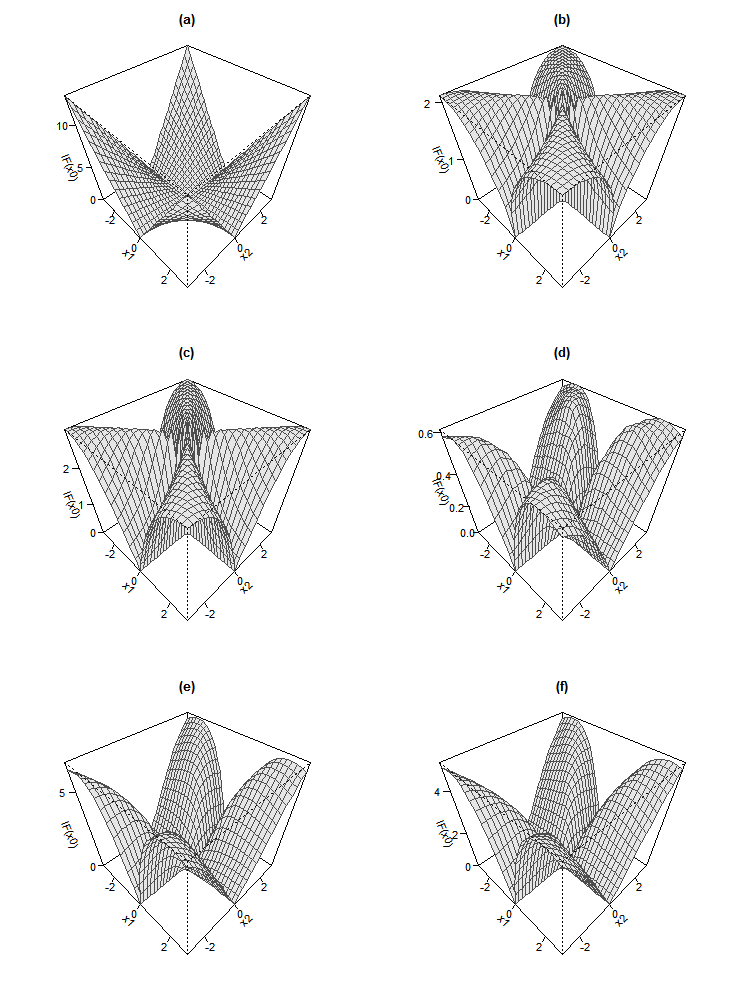
\includegraphics[width=12cm]{../Codes/IFnorm.png}
	\caption{Plot of the norm of influence function for first eigenvector of (a) sample covariance matrix, (b) SCM, (c) Tyler's scatter matrix and DCMs for (d) Halfspace depth, (e) Mahalanobis depth, (f) Projection depth for a bivariate normal distribution with $\bfmu = {\bf 0}, \Sigma = \diag(2,1)$}
	\label{fig:IFnorm}
\end{figure}

In Figure \ref{fig:IFnorm} we consider first eigenvectors of our scatter estimates, as well as teo well-known robust estimates of scatter: the Sign Covariance Matrix (SCM) and Tyler's shape matrix, for the $\mathcal{N}_2((0,0)^T, \diag(2,1))$ and plot norms of these influence functions for different values of $\bfx_0$. Influence function for the $i^\text{th}$ eigenvectors of these two matrices (say $\bfgamma_{S,i}$ and $\bfgamma_{T,i}$, respectively) are as follows:
%
\begin{eqnarray*}
\quad IF(\bfx_0; \bfgamma_{S,i}, F) &=& \sum_{k=1; k \neq i}^p \frac{\sqrt{\lambda_i \lambda_k}}{\lambda_{S,i} - \lambda_{S,k}}. \frac{z_{0i} z_{0k}}{\bfz_0^T \Lambda \bfz_0} \bfgamma_k, \text{ with } \lambda_{S,i} = E_\bfZ \left( \frac{\lambda_i z_i^2}{\sum_{j=1}^p \lambda_j z_j^2} \right) \quad \\
IF(\bfx_0; \bfgamma_{T,i}, F) &=& (p+2) \sum_{k=1; k \neq i}^p \frac{\sqrt{\lambda_i \lambda_k}}{\lambda_i - \lambda_k}. \frac{z_{0i} z_{0k}}{\bfz_0^T \bfz_0} \bfgamma_k \quad 
\end{eqnarray*}
%
Their corresponding plots demonstrate the 'inlier effect', i.e. points close to symmetry center and the center itself having high influence, which results in loss of efficiency. The influence function for the sample covariance matrix is obtained by replacing $(p+2)$ by $\| \bfz_0 \|^2$ in the expression of $IF(\bfx_0; \bfgamma_{T,i}, F)$ above, hence is unbounded and the corresponding eigenvector estimators are not robust. In comparison, all three DCMs considered here have a bounded influence function as well as small values of the influence function at 'deep' points.

\subsubsection{Asymptotic and finite-sample efficiencies}

%Unlike affine equivariant estimators of shape, the Asymptotic Relative Efficiency (ARE) of eigenvectors (with respect to any other affine equivariant estimator) can not be simplified as a ratio of two scalar quantities dependent on only the distribution of $\| \bfz \|$ (e.g. \cite{taskinen12,ollilia03}).
Suppose $\hat C$ is a $\sqrt n$-consistent estimator of a scatter functional $C$. Then the asymptotic variance of its eigenvectors are \cite{anderson}
%
\begin{equation} \label{equation:covevEq}
AVar(\sqrt n\hat \bfgamma_{c,i}) = \sum_{k=1; k \neq i}^p \frac{\lambda_i \lambda_k}{(\lambda_i - \lambda_k)^2} \bfgamma_k \bfgamma_k^T
\end{equation}
%
The asymptotic relative efficiencies of eigenvectors from the sample DCM with respect to the sample covariance matrix can now be derived using (\ref{equation:covevEq}) above and (\ref{equation:DevEq}) from Corollary \ref{Corollary:eigendist}:
%
\begin{eqnarray*}
ARE(\hat\bfgamma^D_i, \hat\bfgamma_i; F) &=& \frac{\Tr( AVar(\sqrt n\hat \bfgamma_i))}{\Tr( AVar(\sqrt n\hat \bfgamma^D_i))}\\
&=& \left[\sum_{k=1; k \neq i}^p \frac{\lambda_i \lambda_k}{(\lambda_i - \lambda_k)^2} \right] \left[ \sum_{k=1; k \neq i}^p \frac{\lambda_i \lambda_k }{(\lambda_{D,s,i} - \lambda_{D,S,k})^2} E \left( \frac{(D^-_\bfZ (\bfz))^4 z_i^2 z_k^2}{(\bfz^T \Lambda \bfz)^2} \right) \right]^{-1}
\end{eqnarray*}

Obtaining ARE of the ADCM is, in comparison to DCM, more straightforward. The asymptotic covariance matrix of an eigenvector of the affine equivariant scatter functional $C$ is given by:
%
$$
AVar (\sqrt n  \hat\bfgamma_{C,j}) = ASV (C_{12}, F_0) \sum_{k=1, k \neq i}^p \frac{\lambda_i \lambda_k}{\lambda_i - \lambda_k}. \bfgamma_i \bfgamma_k^T
$$
%
where $ASV (C_{12}, F_0)$ is the asymptotic variance of an off-diagonal element of $C$ when the underlying distribution is $F_0$. Following \cite{croux00} this equals
%
$$
ASV (C_{12}, F_0) = E_{F_0} \left[ \alpha_c (\| \bfz \|)^2 (S_1(\bfz)S_2 (\bfz))^2 \right] = E_{F_0} \alpha_C (\| \bfz \|)^2 . E_{F_0} (S_1(\bfz)S_2 (\bfz))^2 
$$
% 
again using the fact that $\|\bfZ\|$ and $\bfS(\bfZ)$ are independent with $\bfZ \sim F_0$. It now follows that
%
\begin{equation}
ARE (\hat\bfgamma_{\Sigma_M,i}, \hat\bfgamma_{Cov,i}; F) = \frac{E_{F_0} \alpha_{Cov} (\| \bfz \|)^2}{E_{F_0} \alpha_C (\| \bfz \|)^2} = \frac{E_{F_0} \| \bfz \|^4. \left[ E_{F_0} ( p u \| \bfz\| + u'( \| \bfz \|) \| \bfz \| ) \right]^2}{E_{F_0} (u(\| \bfz \|))^2}
\end{equation}
%

Table \ref{table:AREtable} considers 6 different elliptic distributions (namely, bivariate $t$ with df = 5, 6, 10, 15, 25 and bivariate normal) and summarizes ARE for first eigenvectors for ADCMs corresponding to projection depth (PD-ACM) and halfspace depth (HSD-ACM). Due to difficulty of analytically obtain the AREs, we calculate them using Monte-Carlo simulation of $10^6$ samples and subsequent numerical integration. The ADCM seems to be particularly efficient in lower dimensions for distributions with heavier tails ($t_5$ and $t_6$), while for distributions with lighter tails, the AREs increase with data dimension. At higher values of $p$ the ADCM is almost as efficient as the sample covarnace matrix when the data comes from multivariate normal distribution.

\begin{table}[t]
\centering
    \begin{tabular}{c|cccc|cccc}
    \hline
    & \multicolumn{4}{c|}{PD-ACM} & \multicolumn{4}{c}{HSD-ACM} \\\cline{2-9}
    Distribution & $p=2$  & $p=5$  & $p=10$ & $p=20$ & $p=2$  & $p=5$  & $p=10$ & $p=20$ \\ \hline
    $t_5$           & 4.73 & 3.99 & 3.46 & 3.26 & 4.18 & 3.63 & 3.36 & 3.15 \\
    $t_6$           & 2.97 & 3.28 & 2.49 & 2.36 & 2.59 & 2.45 & 2.37 & 2.32 \\
    $t_{10}$          & 1.45 & 1.47 & 1.49 & 1.52 & 1.30 & 1.37 & 1.43 & 1.49 \\
    $t_{15}$          & 1.15 & 1.19 & 1.23 & 1.27 & 1.01 & 1.10 & 1.17 & 1.24 \\
    $t_{25}$          & 0.97 & 1.02 & 1.07 & 1.11 & 0.85 & 0.94 & 1.02 & 1.08 \\
    MVN          & 0.77 & 0.84 & 0.89 & 0.93 & 0.68 & 0.77 & 0.84 & 0.91 \\ \hline
    \end{tabular}
    \caption{Table of AREs of the ADCM for different choices of $p$ and data-generating distributions, and two choices of depth functions}
    \label{table:AREtable}
\end{table}

We now obtain finite sample efficiencies of the three DCMs as well as their depth-weighted affine equivariant counterparts by a simulation study, and compare them with the same from the SCM and Tyler's scatter matrix. We consider the same 6 elliptical distributions considered in ARE calculations above, and from every distribution draw 10000 samples each for sample sizes $n = 20, 50, 100, 300, 500$. All distributions are centered at ${\bf 0}_p$, and have covariance matrix $\Sigma = \diag(p,p-1,...1)$. We consider 3 choices of $p$: 2, 3 and 4.

We use the concept of principal angles \citep{miao92} to find out error estimates for the first eigenvector of a scatter matrix. In our case, the first eigenvector will be
%
$$ \bfgamma_1 = (1,\overbrace{0,...,0}^{p-1})^T $$
%
For an estimate of the eigenvector, say $\hat\bfgamma_1$, error in prediction is measured by the smallest angle between the two lines, i.e. $ \cos^{-1} | \hat\bfgamma_1^T \hat\bfgamma_1 | $. A smaller absolute value of this angle is equivalent to better prediction. We repeat this 10000 times and calculate the \textbf{Mean Squared Prediction Angle}:
%
$$ MSPA(\hat \bfgamma_1) = \frac{1}{10000} \sum_{m=1}^{10000} \left( \cos^{-1} \left|\bfgamma_1^T \hat\bfgamma^{(m)}_1 \right| \right)^2 $$
%
Finally, the finite sample efficiency of some eigenvector estimate $\hat\bfgamma^E_1$ relative to that obtained from the sample covariance matrix, say $\hat\bfgamma^{Cov}_1$ is obtained as:
$$ FSE(\hat\bfgamma^E_1, \hat\bfgamma^{Cov}_1) = \frac{MSPA(\hat\bfgamma^{Cov}_1)}{MSPA(\hat\bfgamma^E_1)} $$

Tables \ref{table:FSEtable2}, \ref{table:FSEtable3} and \ref{table:FSEtable4} give FSE values for $p=2,3,4$, respectively. In general, all the efficiencies increase as the dimension $p$ goes up. DCM-based estimators (columns 3-5 in each table) outperform SCM and Tyler's scatter matrix, and among the 3 depths considered, projection depth seems to give the best results. Its finite sample performances are better than Tyler's and Huber's M-estimators of scatter as well as their symmetrized counterparts (see Table 4 in \cite{sirkia07}, and quite close to the affine equivariant spatial sign covariance matrix (see Table 2 in \cite{ollilia03}). The depth-weighted iterated versions of these 3 SCMs (columns 6-8 in each table) seem to further better the performance of their corresponding orthogonal equivariant counterparts.

\begin{table}[b]
\begin{footnotesize}
    \begin{tabular}{c|cc|ccc|ccc}
    \hline
    $F$ = Bivariate $t_5$    & SCM  & Tyler & HSD-CM & MhD-CM & PD-CM & HSD-wCM & MhD-wCM & PD-wCM \\ \hline
    $n$=20                   & 0.80 & 0.83  & 0.95   & 0.95   & 0.89  & 1.00    & 0.96    & 0.89   \\
    $n$=50                   & 0.86 & 0.90  & 1.25   & 1.10   & 1.21  & 1.32    & 1.13    & 1.25   \\
    $n$=100                  & 1.02 & 1.04  & 1.58   & 1.20   & 1.54  & 1.67    & 1.24    & 1.63   \\
    $n$=300                  & 1.24 & 1.28  & 1.81   & 1.36   & 1.82  & 1.93    & 1.44    & 1.95   \\
    $n$=500                  & 1.25 & 1.29  & 1.80   & 1.33   & 1.84  & 1.91    & 1.39    & 1.97   \\ \hline
    $F$ = Bivariate $t_6$    & SCM  & Tyler & HSD-CM & MhD-CM & PD-CM & HSD-wCM & MhD-wCM & PD-wCM \\ \hline
    $n$=20                   & 0.77 & 0.79  & 0.92   & 0.92   & 0.86  & 0.96    & 0.92    & 0.85   \\
    $n$=50                   & 0.76 & 0.78  & 1.11   & 1.00   & 1.08  & 1.17    & 1.03    & 1.13   \\
    $n$=100                  & 0.78 & 0.79  & 1.27   & 1.06   & 1.33  & 1.35    & 1.11    & 1.41   \\
    $n$=300                  & 0.88 & 0.91  & 1.29   & 1.09   & 1.35  & 1.38    & 1.15    & 1.45   \\
    $n$=500                  & 0.93 & 0.96  & 1.37   & 1.13   & 1.40  & 1.44    & 1.19    & 1.48   \\ \hline
    $F$ = Bivariate $t_{10}$ & SCM  & Tyler & HSD-CM & MhD-CM & PD-CM & HSD-wCM & MhD-wCM & PD-wCM \\ \hline
    $n$=20                   & 0.70 & 0.72  & 0.83   & 0.84   & 0.77  & 0.89    & 0.87    & 0.79   \\
    $n$=50                   & 0.58 & 0.60  & 0.90   & 0.84   & 0.86  & 0.95    & 0.88    & 0.91   \\
    $n$=100                  & 0.57 & 0.59  & 0.92   & 0.87   & 0.97  & 0.98    & 0.90    & 1.03   \\
    $n$=300                  & 0.62 & 0.64  & 0.93   & 0.85   & 0.99  & 0.99    & 0.91    & 1.06   \\
    $n$=500                  & 0.62 & 0.65  & 0.93   & 0.86   & 1.00  & 1.00    & 0.92    & 1.08   \\ \hline
    $F$ = Bivariate $t_{15}$ & SCM  & Tyler & HSD-CM & MhD-CM & PD-CM & HSD-wCM & MhD-wCM & PD-wCM \\ \hline
    $n$=20                   & 0.63 & 0.66  & 0.76   & 0.78   & 0.72  & 0.81    & 0.81    & 0.73   \\
    $n$=50                   & 0.52 & 0.52  & 0.79   & 0.75   & 0.80  & 0.84    & 0.79    & 0.85   \\
    $n$=100                  & 0.51 & 0.52  & 0.83   & 0.77   & 0.88  & 0.88    & 0.81    & 0.94   \\
    $n$=300                  & 0.55 & 0.56  & 0.84   & 0.79   & 0.91  & 0.89    & 0.84    & 0.98   \\
    $n$=500                  & 0.56 & 0.59  & 0.85   & 0.80   & 0.93  & 0.91    & 0.86    & 0.99   \\ \hline
    $F$ = Bivariate $t_{25}$ & SCM  & Tyler & HSD-CM & MhD-CM & PD-CM & HSD-wCM & MhD-wCM & PD-wCM \\ \hline
    $n$=20                   & 0.63 & 0.65  & 0.77   & 0.79   & 0.74  & 0.80    & 0.81    & 0.74   \\
    $n$=50                   & 0.49 & 0.50  & 0.73   & 0.71   & 0.76  & 0.78    & 0.75    & 0.80   \\
    $n$=100                  & 0.45 & 0.46  & 0.73   & 0.69   & 0.81  & 0.78    & 0.73    & 0.87   \\
    $n$=300                  & 0.51 & 0.52  & 0.78   & 0.75   & 0.87  & 0.83    & 0.79    & 0.94   \\
    $n$=500                  & 0.53 & 0.55  & 0.79   & 0.75   & 0.87  & 0.84    & 0.80    & 0.94   \\ \hline
    $F$ = BVN                & SCM  & Tyler & HSD-CM & MhD-CM & PD-CM & HSD-wCM & MhD-wCM & PD-wCM \\ \hline
    $n$=20                   & 0.56 & 0.60  & 0.69   & 0.71   & 0.67  & 0.73    & 0.74    & 0.68   \\
    $n$=50                   & 0.42 & 0.43  & 0.66   & 0.66   & 0.70  & 0.71    & 0.69    & 0.75   \\
    $n$=100                  & 0.42 & 0.43  & 0.69   & 0.66   & 0.77  & 0.74    & 0.71    & 0.83   \\
    $n$=300                  & 0.47 & 0.49  & 0.71   & 0.69   & 0.82  & 0.76    & 0.73    & 0.88   \\
    $n$=500                  & 0.48 & 0.50  & 0.73   & 0.71   & 0.83  & 0.78    & 0.76    & 0.89   \\ \hline
    \end{tabular}
\end{footnotesize}
\caption{Finite sample efficiencies of several scatter matrices: $p=2$}
\label{table:FSEtable2}
\end{table}

\begin{table}[b]
\begin{footnotesize}
   \begin{tabular}{c|cc|ccc|ccc}
    \hline
    3-variate $t_5$    & SCM  & Tyler & HSD-CM & MhD-CM & PD-CM & HSD-wCM & MhD-wCM & PD-wCM \\ \hline
    $n$=20             & 0.96 & 0.97  & 1.06   & 1.03   & 0.99  & 1.07    & 1.06    & 0.97   \\
    $n$=50             & 1.07 & 1.08  & 1.28   & 1.20   & 1.18  & 1.33    & 1.23    & 1.20   \\
    $n$=100            & 1.12 & 1.15  & 1.49   & 1.31   & 1.40  & 1.57    & 1.38    & 1.48   \\
    $n$=300            & 1.49 & 1.54  & 2.09   & 1.82   & 2.07  & 2.19    & 1.93    & 2.18   \\
    $n$=500            & 1.60 & 1.66  & 2.18   & 1.87   & 2.21  & 2.27    & 1.95    & 2.30   \\ \hline
    3-variate $t_6$    & SCM  & Tyler & HSD-CM & MhD-CM & PD-CM & HSD-wCM & MhD-wCM & PD-wCM \\ \hline
    $n$=20             & 0.90 & 0.92  & 1.00   & 0.99   & 0.95  & 1.02    & 1.01    & 0.94   \\
    $n$=50             & 0.95 & 0.96  & 1.16   & 1.09   & 1.09  & 1.21    & 1.14    & 1.11   \\
    $n$=100            & 0.98 & 0.99  & 1.32   & 1.22   & 1.25  & 1.38    & 1.27    & 1.29   \\
    $n$=300            & 1.10 & 1.14  & 1.57   & 1.40   & 1.58  & 1.62    & 1.47    & 1.64   \\
    $n$=500            & 1.17 & 1.20  & 1.57   & 1.43   & 1.60  & 1.63    & 1.51    & 1.67   \\ \hline
    3-variate $t_{10}$ & SCM  & Tyler & HSD-CM & MhD-CM & PD-CM & HSD-wCM & MhD-wCM & PD-wCM \\ \hline
    $n$=20             & 0.87 & 0.88  & 0.95   & 0.94   & 0.90  & 0.97    & 0.98    & 0.89   \\
    $n$=50             & 0.77 & 0.79  & 0.96   & 0.92   & 0.94  & 0.99    & 0.96    & 0.95   \\
    $n$=100            & 0.75 & 0.76  & 1.02   & 0.95   & 1.01  & 1.06    & 1.00    & 1.05   \\
    $n$=300            & 0.73 & 0.75  & 1.03   & 0.98   & 1.10  & 1.08    & 1.03    & 1.15   \\
    $n$=500            & 0.73 & 0.76  & 1.02   & 0.98   & 1.09  & 1.06    & 1.02    & 1.14   \\ \hline
    3-variate $t_{15}$ & SCM  & Tyler & HSD-CM & MhD-CM & PD-CM & HSD-wCM & MhD-wCM & PD-wCM \\ \hline
    $n$=20             & 0.84 & 0.86  & 0.92   & 0.92   & 0.89  & 0.94    & 0.94    & 0.87   \\
    $n$=50             & 0.75 & 0.76  & 0.92   & 0.90   & 0.90  & 0.96    & 0.94    & 0.93   \\
    $n$=100            & 0.66 & 0.67  & 0.91   & 0.87   & 0.95  & 0.96    & 0.92    & 1.00   \\
    $n$=300            & 0.61 & 0.64  & 0.90   & 0.87   & 1.00  & 0.93    & 0.91    & 1.04   \\
    $n$=500            & 0.65 & 0.67  & 0.89   & 0.87   & 0.99  & 0.93    & 0.91    & 1.03   \\ \hline
    3-variate $t_{25}$ & SCM  & Tyler & HSD-CM & MhD-CM & PD-CM & HSD-wCM & MhD-wCM & PD-wCM \\ \hline
    $n$=20             & 0.78 & 0.79  & 0.87   & 0.89   & 0.87  & 0.89    & 0.92    & 0.86   \\
    $n$=50             & 0.70 & 0.71  & 0.88   & 0.86   & 0.88  & 0.91    & 0.90    & 0.90   \\
    $n$=100            & 0.61 & 0.63  & 0.86   & 0.83   & 0.89  & 0.90    & 0.88    & 0.94   \\
    $n$=300            & 0.58 & 0.59  & 0.83   & 0.80   & 0.92  & 0.87    & 0.85    & 0.98   \\
    $n$=500            & 0.62 & 0.64  & 0.83   & 0.82   & 0.94  & 0.88    & 0.87    & 0.99   \\ \hline
    3-variate Normal   & SCM  & Tyler & HSD-CM & MhD-CM & PD-CM & HSD-wCM & MhD-wCM & PD-wCM \\ \hline
    $n$=20             & 0.76 & 0.78  & 0.85   & 0.87   & 0.84  & 0.87    & 0.90    & 0.83   \\
    $n$=50             & 0.66 & 0.67  & 0.82   & 0.81   & 0.84  & 0.86    & 0.86    & 0.86   \\
    $n$=100            & 0.56 & 0.58  & 0.77   & 0.75   & 0.83  & 0.82    & 0.79    & 0.87   \\
    $n$=300            & 0.53 & 0.55  & 0.75   & 0.74   & 0.85  & 0.79    & 0.78    & 0.90   \\
    $n$=500            & 0.56 & 0.58  & 0.76   & 0.76   & 0.87  & 0.80    & 0.80    & 0.92   \\ \hline
    \end{tabular}
\end{footnotesize}
\caption{Finite sample efficiencies of several scatter matrices: $p=3$}
\label{table:FSEtable3}
\end{table}

\begin{table}[b]
\begin{footnotesize}
    \begin{tabular}{c|cc|ccc|ccc}
    \hline
    4-variate $t_5$    & SCM  & Tyler & HSD-CM & MhD-CM & PD-CM & HSD-wCM & MhD-wCM & PD-wCM \\ \hline
    $n$=20             & 1.04 & 1.02  & 1.10   & 1.07   & 1.02  & 1.09    & 1.07    & 0.98   \\
    $n$=50             & 1.08 & 1.08  & 1.16   & 1.16   & 1.13  & 1.19    & 1.19    & 1.13   \\
    $n$=100            & 1.31 & 1.31  & 1.42   & 1.38   & 1.36  & 1.46    & 1.44    & 1.36   \\
    $n$=300            & 1.46 & 1.54  & 1.81   & 1.76   & 1.95  & 1.88    & 1.88    & 1.95   \\
    $n$=500            & 1.92 & 1.93  & 2.23   & 2.03   & 2.31  & 2.35    & 2.19    & 2.39   \\ \hline
    4-variate $t_6$    & SCM  & Tyler & HSD-CM & MhD-CM & PD-CM & HSD-wCM & MhD-wCM & PD-wCM \\ \hline
    $n$=20             & 1.00 & 1.05  & 1.03   & 1.05   & 1.00  & 1.04    & 1.04    & 0.95   \\
    $n$=50             & 1.03 & 1.01  & 1.13   & 1.12   & 1.11  & 1.19    & 1.17    & 1.10   \\
    $n$=100            & 1.08 & 1.12  & 1.25   & 1.23   & 1.27  & 1.24    & 1.25    & 1.22   \\
    $n$=300            & 1.34 & 1.36  & 1.64   & 1.52   & 1.60  & 1.67    & 1.61    & 1.68   \\
    $n$=500            & 1.26 & 1.34  & 1.55   & 1.49   & 1.60  & 1.65    & 1.61    & 1.69   \\ \hline
    4-variate $t_{10}$ & SCM  & Tyler & HSD-CM & MhD-CM & PD-CM & HSD-wCM & MhD-wCM & PD-wCM \\ \hline
    $n$=20             & 0.90 & 0.89  & 0.95   & 0.98   & 0.98  & 0.96    & 1.01    & 0.95   \\
    $n$=50             & 0.90 & 0.91  & 1.01   & 0.98   & 0.98  & 1.03    & 1.04    & 0.99   \\
    $n$=100            & 0.87 & 0.87  & 0.93   & 0.95   & 1.01  & 0.99    & 1.01    & 1.05   \\
    $n$=300            & 0.87 & 0.87  & 1.09   & 1.09   & 1.17  & 1.14    & 1.16    & 1.23   \\
    $n$=500            & 0.88 & 0.92  & 1.10   & 1.10   & 1.23  & 1.19    & 1.22    & 1.29   \\ \hline
    4-variate $t_{15}$ & SCM  & Tyler & HSD-CM & MhD-CM & PD-CM & HSD-wCM & MhD-wCM & PD-wCM \\ \hline
    $n$=20             & 0.92 & 0.90  & 0.94   & 0.94   & 0.96  & 0.95    & 0.97    & 0.89   \\
    $n$=50             & 0.82 & 0.83  & 0.88   & 0.91   & 0.93  & 0.88    & 0.93    & 0.93   \\
    $n$=100            & 0.84 & 0.87  & 0.92   & 0.95   & 1.00  & 0.93    & 0.96    & 1.00   \\
    $n$=300            & 0.73 & 0.75  & 0.96   & 0.99   & 1.10  & 1.00    & 1.06    & 1.12   \\
    $n$=500            & 0.73 & 0.76  & 0.95   & 0.96   & 1.06  & 0.94    & 0.97    & 1.06   \\ \hline
    4-variate $t_{25}$ & SCM  & Tyler & HSD-CM & MhD-CM & PD-CM & HSD-wCM & MhD-wCM & PD-wCM \\ \hline
    $n$=20             & 0.89 & 0.92  & 0.92   & 0.92   & 0.90  & 0.96    & 0.95    & 0.89   \\
    $n$=50             & 0.82 & 0.84  & 0.89   & 0.90   & 0.91  & 0.93    & 0.96    & 0.92   \\
    $n$=100            & 0.77 & 0.76  & 0.90   & 0.90   & 0.96  & 0.94    & 0.98    & 1.04   \\
    $n$=300            & 0.73 & 0.77  & 0.93   & 0.91   & 0.98  & 1.00    & 0.98    & 1.03   \\
    $n$=500            & 0.67 & 0.71  & 0.83   & 0.83   & 0.96  & 0.88    & 0.90    & 1.00   \\ \hline
    4-variate Normal   & SCM  & Tyler & HSD-CM & MhD-CM & PD-CM & HSD-wCM & MhD-wCM & PD-wCM \\ \hline
    $n$=20             & 0.82 & 0.84  & 0.87   & 0.90   & 0.91  & 0.89    & 0.93    & 0.89   \\
    $n$=50             & 0.80 & 0.81  & 0.87   & 0.88   & 0.88  & 0.88    & 0.92    & 0.88   \\
    $n$=100            & 0.68 & 0.71  & 0.80   & 0.85   & 0.91  & 0.82    & 0.86    & 0.92   \\
    $n$=300            & 0.61 & 0.63  & 0.82   & 0.85   & 0.93  & 0.86    & 0.91    & 0.96   \\
    $n$=500            & 0.60 & 0.64  & 0.77   & 0.80   & 0.90  & 0.82    & 0.86    & 0.96   \\ \hline
    \end{tabular}
\end{footnotesize}
\caption{Finite sample efficiencies of several scatter matrices: $p=4$}
\label{table:FSEtable4}
\end{table}

\subsection{Robust estimation of eigenvalues, and a plug-in estimator of $\Sigma$}

As we have seen in theorem \ref{Theorem:covform}, eigenvalues of the DCM are not same as the population eigenvalues, whereas the ADCM only gives back standardized eigenvalues. However, it is possible to robustly estimate the original eigenvalues by working with the individual columns of the robust score matrix. We do this using the following steps:

\begin{enumerate}
\item Randomly divide the sample indices $\{1,2,...,n\}$ into $k$ disjoint groups $\{G_1,...,G_k \}$ of size $\lfloor n/k \rfloor$ each;

\item Assume the data is centered. Transform the data matrix: $S = \hat\Gamma^T_D X$;

\item Calculate coordinate-wise variances for each group of indices $G_j$:
%
$$
\hat\lambda_{i,j} = \frac{1}{|G_j|} \sum_{l \in G_j} (s_{li} - \bar s_{G_j,i})^2; \quad i = 1,...,p; j = 1,...,k
$$
where $\bar\bfs_{G_j} = (\bar s_{G_j,1}, ..., \bar s_{G_j,p})^T$ is the vector of column-wise means of $S_{G_j}$, the submatrix od $S$ with row indices in $G_j$.
%
\item Obtain estimates of eigenvalues by taking coordinate-wise medians of these variances:
%
$$
\hat \lambda_i = \text{median} (\hat\lambda_{i,1}, ... , \hat\lambda_{i,k} ); \quad i = 1,...,p
$$
%
\end{enumerate}
%
The number of subgroups used to calculate this median-of-small-variances estimator can be determined following \citep{Minsker15}. After this, we construct a consistent plug-in estimator of the population covariance matrix $\Sigma$:

\begin{Theorem}\label{Thm:pluginSigma}
Consider the estimates $\hat\lambda_i$ obtained from the above algorithm, and the matrix of eigenvectors $\hat\Gamma_D$ estimated using the sample DCM. Define $\hat\Sigma = \hat\Gamma_D \hat\Lambda \hat\Gamma_D^T; \hat\Lambda = \text{diag}(\hat\lambda_1, ..., \hat\lambda_p)$. Then as $n \rightarrow \infty$,
%
$$ \| \hat\Sigma - \Sigma \|_F \stackrel{P}{\rightarrow} 0 $$
%
$\|.\|_F$ being the Frobenius norm.
\end{Theorem}

{\colrbf (put in 1 or 2 sentences?)}
